\documentclass[12pt, a4paper]{article}
% Seznam balíků
\usepackage{comment}
\usepackage{lmodern}
\usepackage{cmap}
\usepackage[czech]{babel}
\usepackage[T1]{fontenc}
\usepackage[utf8]{inputenc}
\usepackage{graphicx}
\usepackage{epstopdf}
\usepackage{makeidx}
\usepackage{listings}
\usepackage[export]{adjustbox}
\usepackage[font=scriptsize,labelfont=bf]{caption}
\usepackage{booktabs}
\usepackage{subcaption}
\usepackage{array}
\usepackage{multirow}
\usepackage{enumitem}
\usepackage{tocbibind}
\usepackage{courier}
\usepackage{pdfpages}
\usepackage{hyperref}
\hypersetup{
	colorlinks,
	citecolor=black,
	filecolor=black,
	linkcolor=black,
	urlcolor=black
}

% Začátek dokumentu
\begin{document}
	% Titulní stránka
	\begin{titlepage}
		\centering
		\begin{tabular}{m{0.2\linewidth}m{0.8\linewidth}}
			
\includegraphics[width=1\linewidth]{SPSE_logo.png}
			&\centering
			\textbf{Vyšší odborná škola}\par
			\textbf{a Střední průmyslová škola elektrotechnická}\par
			\textbf{Plzeň, Koterovská 85}
		\end{tabular}
		\centering
		\vfill
		{\Huge\scshape Ročníková práce\par}
		\raggedright
		\vspace{4cm}
		{\Large Téma: Programovatelné auto\par}
		\vfill
		
		% Spodní část titulní stránky
		\begin{tabular}{ll}
			Autor práce:		&	Jan Ocelík \\
			Obor studia:		&	78-42-M/01 Technické lyceum \\
			Třída:				&	3. L \\
			Předmět:			&	Kybernetika \\
			Zadávající učitel:	&	Jiří Švihla \\
			Dne:				&	28. 4. 2023 \\
								&	\\
			Hodnocení:			&	\\
		\end{tabular}
	\end{titlepage}
	
	% Zadání
	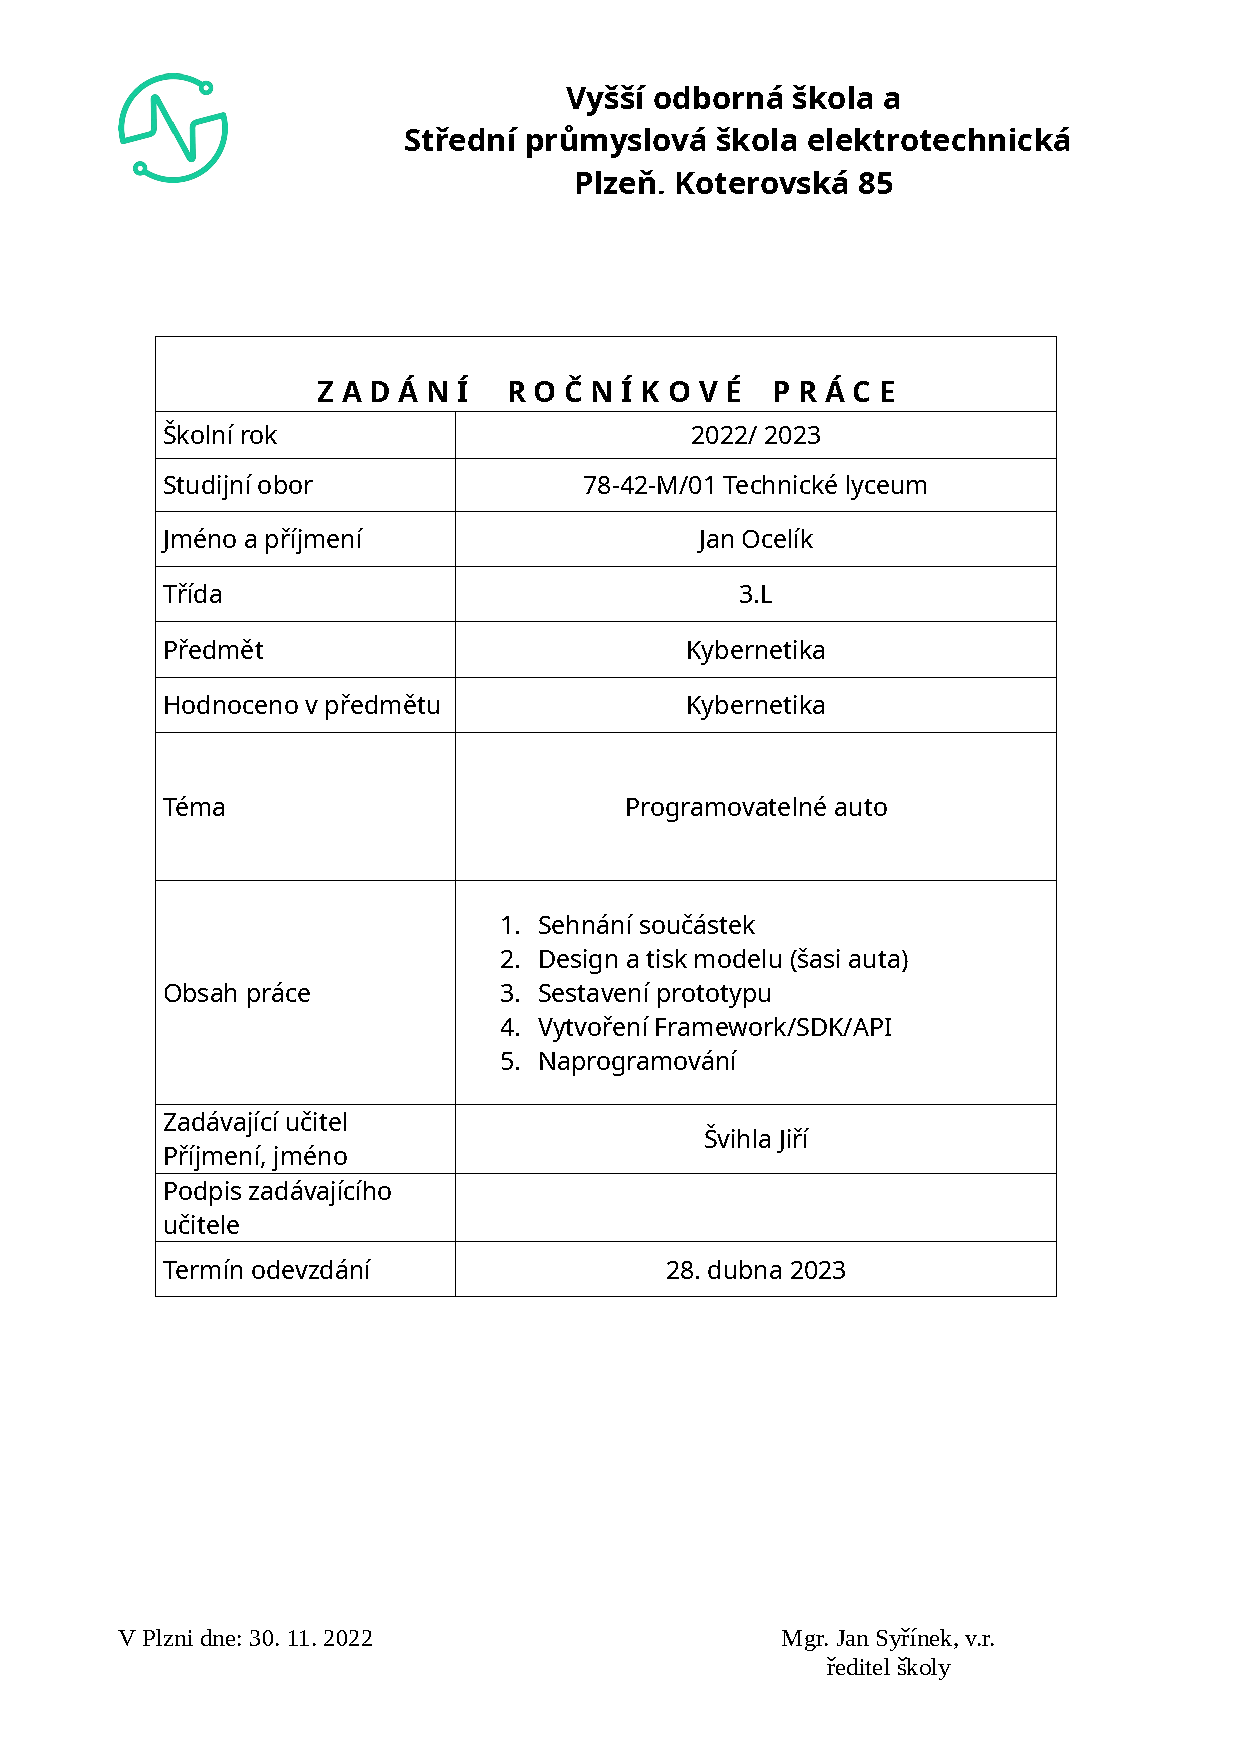
\includepdf[pages=-]{Zadani_RP_TL_22_23.pdf}
	\thispagestyle{empty}
	
	% Anotace
	\newpage
	\thispagestyle{empty}
	\section*{Anotace}
	\addcontentsline{toc}{section}{Anotace}
	\paragraph{} Cílem této ročníkové práce je za pomoci opensource programů navrhnout a z opensource komponent poskládat robotické autíčko pro začátečníky i pokročilé s možností jednoduchého sestavení. Dalším úkolem je vyvinout firmware a API pro jednoduché skriptové programovaní i komplexnější programování s využitím obrazového vstupu. Dalším úkolem je připravit úkázkové příklady kódu k předvedení jednotlivých funkčí robota. Posledním úkolem je zpříjemnit práci s robotem, zhodnotit přínosy a možnosti využití projektu ve vzdělávání a vypracovat potřebnou dokumentaci.
	\vfill
	\paragraph{} „Prohlašuji, že jsem tuto práci vypracoval samostatně a použil literárních pramenů a informací, které cituji a uvadím v seznamu použité literatury a zdrojů informací.“
	\paragraph{} „Souhlasím s využitím mé práce učteli VOŠ a SPŠE Plzeň k výuce.“
	\paragraph{} \hfill Plzni dne: .................... Podpis: ....................
	
	% Poděkování
	\newpage
	\thispagestyle{empty}
	\section*{Poděkování}
	\addcontentsline{toc}{section}{Poděkování}
	\paragraph{} Tímto bych chtěl poděkovat vedoucímu práce Jiřímu Švihlovi za pomoc s výběrem komponent a obsahem dokumentace a rodině a přátelům za psychickou podporu. Také děkuji všem dohromady za to, že mě k tomu včas dokopali.
	
	% Obsah
	\newpage
	\tableofcontents
	
	% Úvod
	\newpage
	\section*{Úvod}
	\addcontentsline{toc}{section}{Úvod}
	\paragraph{} V dnešní době se stále více hovoří o automatizaci a digitalizaci a tyto trendy mají velký vliv na společnost. Robotika a autonomní systémy jsou jednou z klíčových oblastí, které se rozvíjejí v rámci těchto trendů a mají potenciál změnit mnoho aspektů našeho života.
	\paragraph{} Vzdělávání a výuka v této oblasti se také stávají stále důležitějšími, protože mnoho pracovních pozic, které budou v budoucnosti vyžadovat znalosti robotiky a programování, ještě neexistuje. Výuka v této oblasti tak může být klíčová pro přípravu studentů na pracovní trh budoucnosti.
	\paragraph{} Proto jsem se rozhodl věnovat svou ročníkovou práci právě problematicerobotiky a vytvořit autonomní auto, které bude sloužit jako výuková pomůcka. Můj záměr je ukázat, jak moderní technologie mohou být využity k tomu, aby byly studenti lépe připraveni na budoucí výzvy v oblasti robotiky a informatiky.
	\paragraph{} Při tvorbě prototypu se budu snažit využít nejnovější poznatky v oblasti robotiky a programování, a to jak z teoretického hlediska, tak z praktického testování. Cílem bude vytvořit zařízení, které bude snadno ovladatelné a srozumitelné pro studenty různých věkových kategorií, a zároveň bude dostatečně funkční a výkonné pro splnění zadaných úkolů.
	\paragraph{} Věřím, že tato ročníková práce přispěje k popularizaci robotiky a podpoří zájem studentů o tuto oblast. Tím může mít pozitivní vliv na jejich budoucí kariéru a na rozvoj robotiky v České republice.
	
	% Cíle a požadavky
	\newpage
	\section{Cíle a požadavky}
	\paragraph{} Lorem ipsum dolor sit amet, consectetuer adipiscing elit. Donec vitae arcu. Maecenas fermentum, sem in pharetra pellentesque, velit turpis volutpat ante, in pharetra metus odio a lectus. Phasellus rhoncus. Class aptent taciti sociosqu ad litora torquent per conubia nostra, per inceptos hymenaeos. Maecenas libero. Aliquam ante. Nullam dapibus fermentum ipsum. Quisque tincidunt scelerisque libero. Aliquam id dolor. Donec quis nibh at felis congue commodo. Suspendisse sagittis ultrices augue. Mauris elementum mauris vitae tortor. Vivamus porttitor turpis ac leo. Sed vel lectus. Donec odio tempus molestie, porttitor ut, iaculis quis, sem. Ut enim ad minima veniam, quis nostrum exercitationem ullam corporis suscipit laboriosam, nisi ut aliquid ex ea commodi consequatur?
	\paragraph{} Class aptent taciti sociosqu ad litora torquent per conubia nostra, per inceptos hymenaeos. Maecenas lorem. Fusce wisi. Fusce nibh. Mauris elementum mauris vitae tortor. Nullam sapien sem, ornare ac, nonummy non, lobortis a enim. Maecenas lorem. Pellentesque pretium lectus id turpis. Maecenas libero. Fusce tellus. Fusce nibh. Aenean fermentum risus id tortor. Mauris dictum facilisis augue. Curabitur vitae diam non enim vestibulum interdum. Duis aute irure dolor in reprehenderit in voluptate velit esse cillum dolore eu fugiat nulla pariatur.
	\paragraph{} Cum sociis natoque penatibus et magnis dis parturient montes, nascetur ridiculus mus. Maecenas sollicitudin. Pellentesque ipsum. Donec quis nibh at felis congue commodo. Etiam dui sem, fermentum vitae, sagittis id, malesuada in, quam. Duis bibendum, lectus ut viverra rhoncus, dolor nunc faucibus libero, eget facilisis enim ipsum id lacus. Quisque tincidunt scelerisque libero. Donec iaculis gravida nulla. Vestibulum fermentum tortor id mi. Cras elementum. Integer lacinia. Duis bibendum, lectus ut viverra rhoncus, dolor nunc faucibus libero, eget facilisis enim ipsum id lacus. Mauris dolor felis, sagittis at, luctus sed, aliquam non, tellus. Nullam rhoncus aliquam metus. Aliquam erat volutpat. Sed vel lectus. Donec odio tempus molestie, porttitor ut, iaculis quis, sem. Etiam neque.
	
	\newpage
	\paragraph{} Aliquam erat volutpat. Fusce aliquam vestibulum ipsum. Vestibulum fermentum tortor id mi. Temporibus autem quibusdam et aut officiis debitis aut rerum necessitatibus saepe eveniet ut et voluptates repudiandae sint et molestiae non recusandae. Ut tempus purus at lorem. Integer pellentesque quam vel velit. Maecenas lorem. Cum sociis natoque penatibus et magnis dis parturient montes, nascetur ridiculus mus. Maecenas aliquet accumsan leo. Vivamus luctus egestas leo. Integer malesuada. Pellentesque sapien. Nullam faucibus mi quis velit. Aliquam erat volutpat. Suspendisse nisl.
\end{document}
% Konec dokumentu
